\chapter{Methodology and Implementation}
\label{chap:metodology}

\section{Blockchain analysis}

Traversing the blockchain is from top to bottom, reason being that blocks only contain the hash of the previous block. 
At a high level the software finds the top block from the chaindata stored in the database and uses it as a starting point.
Then it traverses the transactions in the block and checks if they are relevant for our project, if that is the case they are stored for later use. The hash of the preceding block is used to get it from the database and same process is repeated.
To locate LN relevant transaction we identified attributes they contained not present in other transactions. As stated in chapter 2 \todo{add ref} Lightning channels have an founding/opening and a closing transaction pair. This transaction pair will contain a input - output set of type P2WSH 2of2 mutlsig witch is the channel. This is not sufficent to determine if a transaction is related to the LN or not as P2WSH 2of2 multisig transactions can be used without any relation to the LN. If we look at an arbitrary transaction and see that it has a P2WSH output it can be a founding tx, but we dont even know if the redeem script is a 2of2 multisig script. If we see a transaction which has a 2of2 mutlsig input in its redeem script it might be a closing tx with the possibility of the preceding tx of that input being a founding tx, and that previous transactions possibility of being a founding tx is higher since we now know that the redeem script was a 2of2 multisig script.


\begin{figure}[h]
    \centering
    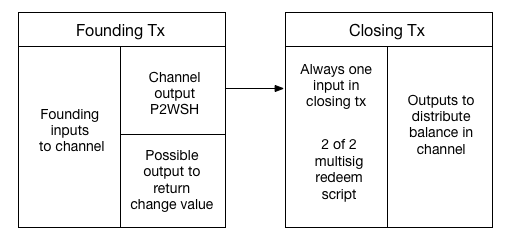
\includegraphics[width=9cm]{figures/lnchain.png}
    \caption{Algorithm of parsing and locating relevant LN transactions on the blockchain}
    \label{fig:htlc_bc}
\end{figure}

\begin{figure}[h]
    \centering
    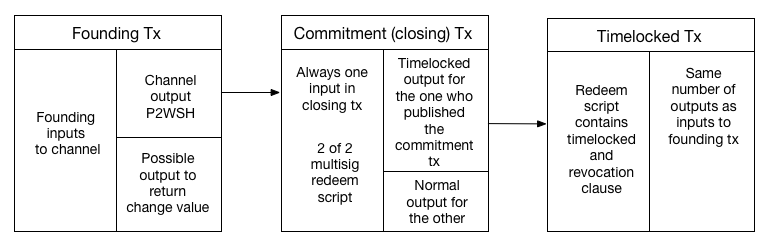
\includegraphics[width=12cm]{figures/lnchainTimelock.png}
    \caption{Algorithm of parsing and locating relevant LN transactions on the blockchain}
    \label{fig:htlc_bc}
\end{figure}

\begin{figure}[h]
    \centering
    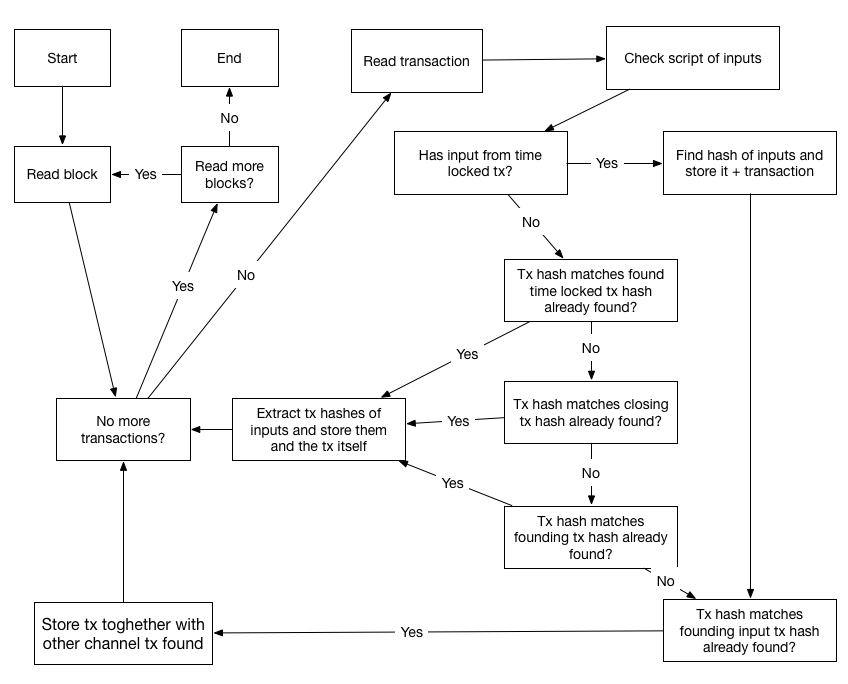
\includegraphics[width=14cm]{figures/algorithm.png}
    \caption{Algorithm of parsing and locating relevant LN transactions on the blockchain}
    \label{fig:htlc_bc}
\end{figure}


\section{Lightning network analysis}
